% Options for packages loaded elsewhere
\PassOptionsToPackage{unicode}{hyperref}
\PassOptionsToPackage{hyphens}{url}
%
\documentclass[
  man,floatsintext]{apa6}
\usepackage{amsmath,amssymb}
\usepackage{lmodern}
\usepackage{iftex}
\ifPDFTeX
  \usepackage[T1]{fontenc}
  \usepackage[utf8]{inputenc}
  \usepackage{textcomp} % provide euro and other symbols
\else % if luatex or xetex
  \usepackage{unicode-math}
  \defaultfontfeatures{Scale=MatchLowercase}
  \defaultfontfeatures[\rmfamily]{Ligatures=TeX,Scale=1}
\fi
% Use upquote if available, for straight quotes in verbatim environments
\IfFileExists{upquote.sty}{\usepackage{upquote}}{}
\IfFileExists{microtype.sty}{% use microtype if available
  \usepackage[]{microtype}
  \UseMicrotypeSet[protrusion]{basicmath} % disable protrusion for tt fonts
}{}
\makeatletter
\@ifundefined{KOMAClassName}{% if non-KOMA class
  \IfFileExists{parskip.sty}{%
    \usepackage{parskip}
  }{% else
    \setlength{\parindent}{0pt}
    \setlength{\parskip}{6pt plus 2pt minus 1pt}}
}{% if KOMA class
  \KOMAoptions{parskip=half}}
\makeatother
\usepackage{xcolor}
\usepackage{graphicx}
\makeatletter
\def\maxwidth{\ifdim\Gin@nat@width>\linewidth\linewidth\else\Gin@nat@width\fi}
\def\maxheight{\ifdim\Gin@nat@height>\textheight\textheight\else\Gin@nat@height\fi}
\makeatother
% Scale images if necessary, so that they will not overflow the page
% margins by default, and it is still possible to overwrite the defaults
% using explicit options in \includegraphics[width, height, ...]{}
\setkeys{Gin}{width=\maxwidth,height=\maxheight,keepaspectratio}
% Set default figure placement to htbp
\makeatletter
\def\fps@figure{htbp}
\makeatother
\setlength{\emergencystretch}{3em} % prevent overfull lines
\providecommand{\tightlist}{%
  \setlength{\itemsep}{0pt}\setlength{\parskip}{0pt}}
\setcounter{secnumdepth}{-\maxdimen} % remove section numbering
% Make \paragraph and \subparagraph free-standing
\ifx\paragraph\undefined\else
  \let\oldparagraph\paragraph
  \renewcommand{\paragraph}[1]{\oldparagraph{#1}\mbox{}}
\fi
\ifx\subparagraph\undefined\else
  \let\oldsubparagraph\subparagraph
  \renewcommand{\subparagraph}[1]{\oldsubparagraph{#1}\mbox{}}
\fi
\newlength{\cslhangindent}
\setlength{\cslhangindent}{1.5em}
\newlength{\csllabelwidth}
\setlength{\csllabelwidth}{3em}
\newlength{\cslentryspacingunit} % times entry-spacing
\setlength{\cslentryspacingunit}{\parskip}
\newenvironment{CSLReferences}[2] % #1 hanging-ident, #2 entry spacing
 {% don't indent paragraphs
  \setlength{\parindent}{0pt}
  % turn on hanging indent if param 1 is 1
  \ifodd #1
  \let\oldpar\par
  \def\par{\hangindent=\cslhangindent\oldpar}
  \fi
  % set entry spacing
  \setlength{\parskip}{#2\cslentryspacingunit}
 }%
 {}
\usepackage{calc}
\newcommand{\CSLBlock}[1]{#1\hfill\break}
\newcommand{\CSLLeftMargin}[1]{\parbox[t]{\csllabelwidth}{#1}}
\newcommand{\CSLRightInline}[1]{\parbox[t]{\linewidth - \csllabelwidth}{#1}\break}
\newcommand{\CSLIndent}[1]{\hspace{\cslhangindent}#1}
\ifLuaTeX
\usepackage[bidi=basic]{babel}
\else
\usepackage[bidi=default]{babel}
\fi
\babelprovide[main,import]{english}
% get rid of language-specific shorthands (see #6817):
\let\LanguageShortHands\languageshorthands
\def\languageshorthands#1{}
% Manuscript styling
\usepackage{upgreek}
\captionsetup{font=singlespacing,justification=justified}

% Table formatting
\usepackage{longtable}
\usepackage{lscape}
% \usepackage[counterclockwise]{rotating}   % Landscape page setup for large tables
\usepackage{multirow}		% Table styling
\usepackage{tabularx}		% Control Column width
\usepackage[flushleft]{threeparttable}	% Allows for three part tables with a specified notes section
\usepackage{threeparttablex}            % Lets threeparttable work with longtable

% Create new environments so endfloat can handle them
% \newenvironment{ltable}
%   {\begin{landscape}\centering\begin{threeparttable}}
%   {\end{threeparttable}\end{landscape}}
\newenvironment{lltable}{\begin{landscape}\centering\begin{ThreePartTable}}{\end{ThreePartTable}\end{landscape}}

% Enables adjusting longtable caption width to table width
% Solution found at http://golatex.de/longtable-mit-caption-so-breit-wie-die-tabelle-t15767.html
\makeatletter
\newcommand\LastLTentrywidth{1em}
\newlength\longtablewidth
\setlength{\longtablewidth}{1in}
\newcommand{\getlongtablewidth}{\begingroup \ifcsname LT@\roman{LT@tables}\endcsname \global\longtablewidth=0pt \renewcommand{\LT@entry}[2]{\global\advance\longtablewidth by ##2\relax\gdef\LastLTentrywidth{##2}}\@nameuse{LT@\roman{LT@tables}} \fi \endgroup}

% \setlength{\parindent}{0.5in}
% \setlength{\parskip}{0pt plus 0pt minus 0pt}

% Overwrite redefinition of paragraph and subparagraph by the default LaTeX template
% See https://github.com/crsh/papaja/issues/292
\makeatletter
\renewcommand{\paragraph}{\@startsection{paragraph}{4}{\parindent}%
  {0\baselineskip \@plus 0.2ex \@minus 0.2ex}%
  {-1em}%
  {\normalfont\normalsize\bfseries\itshape\typesectitle}}

\renewcommand{\subparagraph}[1]{\@startsection{subparagraph}{5}{1em}%
  {0\baselineskip \@plus 0.2ex \@minus 0.2ex}%
  {-\z@\relax}%
  {\normalfont\normalsize\itshape\hspace{\parindent}{#1}\textit{\addperi}}{\relax}}
\makeatother

% \usepackage{etoolbox}
\makeatletter
\patchcmd{\HyOrg@maketitle}
  {\section{\normalfont\normalsize\abstractname}}
  {\section*{\normalfont\normalsize\abstractname}}
  {}{\typeout{Failed to patch abstract.}}
\patchcmd{\HyOrg@maketitle}
  {\section{\protect\normalfont{\@title}}}
  {\section*{\protect\normalfont{\@title}}}
  {}{\typeout{Failed to patch title.}}
\makeatother

\usepackage{xpatch}
\makeatletter
\xapptocmd\appendix
  {\xapptocmd\section
    {\addcontentsline{toc}{section}{\appendixname\ifoneappendix\else~\theappendix\fi\\: #1}}
    {}{\InnerPatchFailed}%
  }
{}{\PatchFailed}
\keywords{keywords\newline\indent Word count: X}
\usepackage{csquotes}
\ifLuaTeX
  \usepackage{selnolig}  % disable illegal ligatures
\fi
\IfFileExists{bookmark.sty}{\usepackage{bookmark}}{\usepackage{hyperref}}
\IfFileExists{xurl.sty}{\usepackage{xurl}}{} % add URL line breaks if available
\urlstyle{same} % disable monospaced font for URLs
\hypersetup{
  pdftitle={Evaluating Machine Translation Performance In Processing Japanese Ellipsis Strategies},
  pdfauthor={Isabelle Chang},
  pdflang={en-EN},
  pdfkeywords={keywords},
  hidelinks,
  pdfcreator={LaTeX via pandoc}}

\title{Evaluating Machine Translation Performance In Processing Japanese Ellipsis Strategies}
\author{Isabelle Chang\textsuperscript{}}
\date{}


\shorttitle{Machine Translation of Japanese Ellipses}

\affiliation{\vspace{0.5cm}\textsuperscript{1} Rutgers University}

\begin{document}
\maketitle

\hypertarget{methods}{%
\section{Methods}\label{methods}}

We report how we determined our sample size, all data exclusions (if any), all manipulations, and all measures in the study.

\hypertarget{participants}{%
\subsection{Participants}\label{participants}}

A total of 14 participants were recruited for this study. Participant age ranged between 19 and 22 years old. All participants were L1 speakers of English, none of which had any formal linguistics training.

\hypertarget{materials}{%
\subsection{Materials}\label{materials}}

\hypertarget{source-sentences}{%
\subsubsection{Source Sentences}\label{source-sentences}}

15 sentences containing one of three ellipsis strategies present in Japanese were generated or selected from existing literature (five for each ellipsis strategy). The three selected strategies were as follows:

\begin{itemize}
\tightlist
\item
  Argument Ellipsis: Also called nominal ellipsis, this
\item
  Verb Phrase Ellipsis-Like constructions:
\item
  Sluicing: A specific type of clausal ellipsis.
\end{itemize}

Japanese sentences were generated with the help of two native Japanese speakers. An intended translation was provided for each sentence to serve as a comparison for the machine-generated translations.

\hypertarget{stimuli---translations}{%
\subsubsection{Stimuli - Translations}\label{stimuli---translations}}

Each of the 15 Japanese sentences was translated using Google, Microsoft Bing, and DeepL Translate (all three services utilize artificial neural networks) for a total of 45 translations.

\hypertarget{acceptability-rating-task}{%
\subsection{Acceptability Rating Task}\label{acceptability-rating-task}}

\hypertarget{procedure}{%
\subsubsection{Procedure}\label{procedure}}

Participants were screened for English proficiency prior to completing this task. For the acceptability rating task, participants were presented with each of the 45 machine-generated translations along with an alphabetical scoring scale (A, D, E, F, G) and asked to assign a score to each translation. Additionally, there were two filler questions presented to the participants halfway and three-quarters of the way through the acceptability rating task.

\hypertarget{scoring}{%
\subsubsection{Scoring}\label{scoring}}

The original alphabetical scoring scale was adopted from \href{https://direct.mit.edu/coli/article/47/4/927/106771/Are-Ellipses-Important-for-Machine-Translation}{Khullar 2021}:

\begin{figure}
\centering
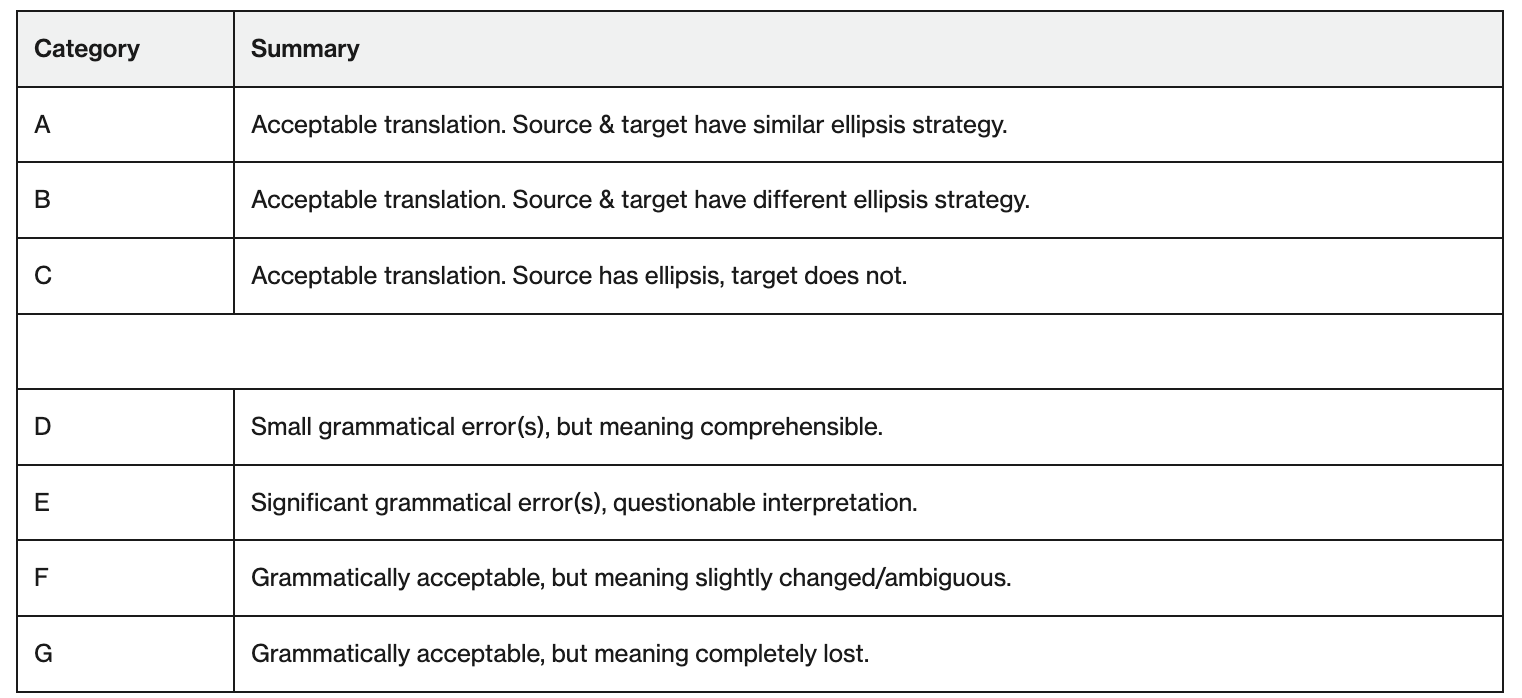
\includegraphics{../figs/alphabetical_scoring.png}
\caption{Alphabetical Scoring Scale}
\end{figure}

For the present study, B and C scores are removed. This was done in part to account for participants' lack of linguistic background. Additionally, argument ellipsis and VPE-like constructs do not exist in English. As such, any grammatical translation in English would not contain these ellipsis strategies, guaranteeing a B or C ranking for Japanese sentences that contain them. The research questions of this project revolve around the accuracy of translation services---that is, how faithfully translation services are able to retain meaning and grammaticality across across Japanese-English translations. As such, B and C scores were replaced with A scores.
Participant-provided alphabetical scores were converted into two sets of numerical scores to quantify the machine translation services' performance on both the meaning and grammaticality of their outputs. The letter-to-number conversion is as follows:

\begin{tabular}{l|r|r}
\hline
alphabetical\_score & meaning\_score & grammaticality\_score\\
\hline
A & 5 & 5\\
\hline
D & 4 & 2\\
\hline
E & 3 & 1\\
\hline
F & 2 & 4\\
\hline
G & 1 & 3\\
\hline
\end{tabular}

The original alphabetical scoring scale only evaluates a translation's faithfulness to the source sentence ellipsis strategy (A-C) and meaning (D-G). Adding another scoring scale for grammaticality allows us to evaluate grammaticality and meaning independently of one another.

\hypertarget{results}{%
\section{Results}\label{results}}

\hypertarget{summary-of-data}{%
\subsection{Summary of Data}\label{summary-of-data}}

14 participants produced 45 acceptability judgments each for a total of 1260 observations (630 for grammaticality and 630 for meaning). Responses to all questions were collected on a Google Form and converted into a .csv file. In the data tidying process, all non-evaluation data were removed. Participant-given alphabetical scores were converted into two separate numerical scores using the system outlined above to yield the following data:

\begin{tabular}{l|l|l|r}
\hline
ellipsis\_type & mt\_service & num\_metric & num\_score\\
\hline
arg & google & meaning & 2\\
\hline
arg & google & grammaticality & 4\\
\hline
arg & google & meaning & 2\\
\hline
arg & google & grammaticality & 4\\
\hline
arg & google & meaning & 5\\
\hline
arg & google & grammaticality & 5\\
\hline
\end{tabular}

\hypertarget{descriptive-statistics}{%
\subsection{Descriptive Statistics}\label{descriptive-statistics}}

Descriptive statistics of acceptability ratings are provided below:

\begin{tabular}{l|r|r}
\hline
ellipsis\_type & grammaticality & meaning\\
\hline
arg & 4.333333 & 3.780952\\
\hline
sluice & 4.076191 & 4.104762\\
\hline
vpel & 3.533333 & 3.314286\\
\hline
\end{tabular}

\hypertarget{data-analysis}{%
\subsection{Data Analysis}\label{data-analysis}}

\hypertarget{discussion}{%
\subsection{Discussion}\label{discussion}}

\newpage

\hypertarget{references}{%
\section{References}\label{references}}

\hypertarget{refs}{}
\begin{CSLReferences}{0}{0}
\end{CSLReferences}


\end{document}
